\documentclass{article}
\usepackage{listings}
\usepackage{xcolor}
\usepackage{tikz}
\usepackage{graphicx}
\usetikzlibrary{shapes, arrows}
\pgfdeclarelayer{background}
\pgfsetlayers{background, main}
\usepackage[margin=0.75in]{geometry}
\title{VHDL Lab 4}
\author{Michael Nolan}

\lstset{
  breaklines=true,
  basicstyle=\ttfamily,
  keywordstyle=\color{green!40!black},
  identifierstyle=\color{blue},
  commentstyle=\color{red!85!black},
  stringstyle=\color{darkgray},
  }



\begin{document}
\maketitle
\newpage

\section{Block diagram}

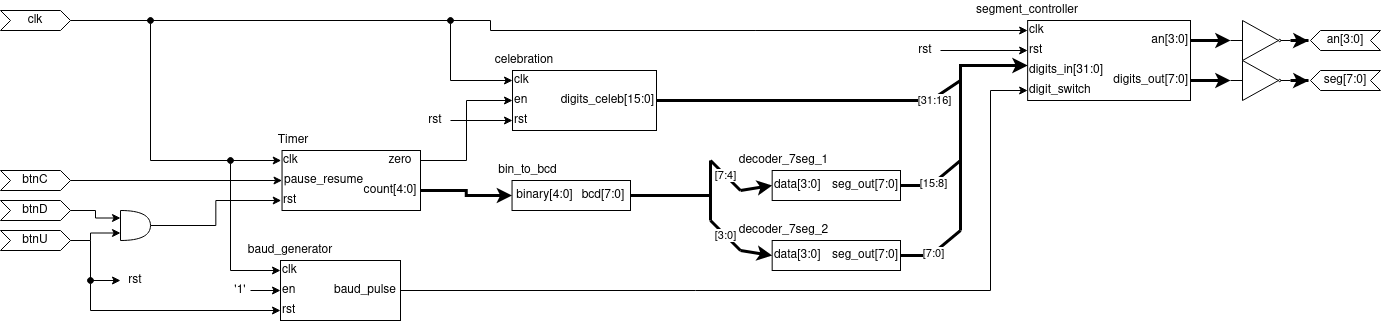
\includegraphics[width=\textwidth]{lab4_diagram}

There really isn't any good software for drawing HDL block diagrams. I've tried tikz, draw.io, and now graphviz, and none are particularly nice. 

\section{VHDL code}
\subsection{lab4.vhd}
\lstinputlisting[language=VHDL]{lab4.vhd}

\subsection{timer.vhd}
\lstinputlisting[language=VHDL]{timer.vhd}

\subsection{baud\_generator.vhd}
\lstinputlisting[language=VHDL]{baud_generator.vhd}

\subsection{bin\_to\_bcd.vhd}
\lstinputlisting[language=VHDL]{bin_to_bcd.vhd}

\subsection{decoder\_7seg.vhd}
\lstinputlisting[language=VHDL]{decoder_7seg.vhd}

\subsection{celebration.vhd}
\lstinputlisting[language=VHDL]{celebration.vhd}

\subsection{segment\_controller.vhd}
\lstinputlisting[language=VHDL]{segment_controller.vhd}

\subsection{types.vhd}
\lstinputlisting[language=VHDL]{types.vhd}

\newpage
\section{Testbench}
\subsection{lab4\_tb.vhd}
\lstinputlisting[language=VHDL]{lab4_tb.vhd}
\subsection{timer\_tb.vhd}
\lstinputlisting[language=VHDL]{timer_tb.vhd}

\newpage
\section{Makefile}
\lstinputlisting[language=make]{Makefile}


\end{document}